\subsection{Performance Comparison on Real-World Clinical Datasets}
\label{sec:exp_clinical}

\begin{table*}[!t]
\centering
\begin{threeparttable}
\caption{Balanced Accuracy (\%) and Friedman Ranks on the 12 Clinical Datasets ($K = 4$, $B = 128$)}
\label{tab:clinical_main}
\scriptsize
\setlength{\tabcolsep}{6.0pt}
\renewcommand{\arraystretch}{1.07}
\begin{tabular}{@{}lrrrr@{\hspace{14pt}}rrrr@{\hspace{14pt}}rr@{}}
\toprule
 & \multicolumn{4}{c}{Aligned Prior} & \multicolumn{4}{c}{Misaligned Prior\tnote{a}} & Mean & \\
\cmidrule(lr{14pt}){2-5} \cmidrule(lr{14pt}){6-9}
Algorithm & $n{=}3$ & $n{=}10$ & $n{=}20$ & $n{=}30$ &
$n{=}3$ & $n{=}10$ & $n{=}20$ & $n{=}30$ & ($n{=}30$) & Rank\tnote{b} \\
\midrule
GA                 & 56.94\rlap{\textsuperscript{*}} & 61.56 & 63.64 & 65.04\rlap{\textsuperscript{*}} & -- & -- & -- & -- & 65.04\rlap{\textsuperscript{*}} & 8.08 \\
BPSO               & 57.42 & 61.52 & 63.47 & 65.35 & -- & -- & -- & -- & 65.35 & 7.42 \\
EDA                & 57.16 & 61.51 & 63.41\rlap{\textsuperscript{*}} & 65.13\rlap{\textsuperscript{*}} & -- & -- & -- & -- & 65.13 & 8.17 \\
MEL                & 57.89 & 62.09 & 63.83 & 65.80 & -- & -- & -- & -- & 65.80 & 7.42 \\
mRMR               & 57.31 & 61.36 & 63.62 & 65.53\rlap{\textsuperscript{*}} & -- & -- & -- & -- & 65.53 & 7.58 \\
ReliefF            & 57.96 & 62.62 & 64.59 & 65.04\rlap{\textsuperscript{*}} & -- & -- & -- & -- & 65.04\rlap{\textsuperscript{*}} & 9.00 \\
L1-LR              & 57.79 & 61.79 & 63.57\rlap{\textsuperscript{*}} & 65.53\rlap{\textsuperscript{*}} & -- & -- & -- & -- & 65.53 & 7.75 \\
RF-Imp             & 57.92 & 61.98 & 64.03 & 65.08 & -- & -- & -- & -- & 65.08 & 7.25 \\
\midrule
$\pi$BO            & 58.03 & 62.40 & 63.98\rlap{\textsuperscript{*}} & 66.21 & 56.78 & 61.38 & 62.90 & 64.74 & 65.48 & 6.25 \\
LLM-Lasso          & 59.04 & 63.09 & 65.01 & 66.30 & 57.04 & 61.39 & 63.30 & 65.16 & 65.73 & 6.33 \\
LSP                & 58.36 & 62.58 & 64.49 & 66.06 & 57.59 & 61.44 & \textbf{63.77} & 65.13 & 65.60 & 6.67 \\
LLM-Select (Rank)  & 60.40 & 64.59 & 66.19 & 66.97 & 54.75\rlap{\textsuperscript{*}} & 57.72\rlap{\textsuperscript{*}} & 59.22 & 59.29\rlap{\textsuperscript{*}} & 63.13\rlap{\textsuperscript{*}} & 10.29 \\
LLM-Select (Score) & \textbf{60.94} & \textbf{65.10} & \textbf{66.90} & \textbf{67.59} & 55.20\rlap{\textsuperscript{*}} & 58.10 & 59.39 & 59.22\rlap{\textsuperscript{*}} & 63.40\rlap{\textsuperscript{*}} & 8.54 \\
\midrule
SP-PD              & 58.66 & 62.54 & 64.68 & 66.65 & \textbf{57.90} & \textbf{61.68} & 63.74 & \textbf{65.85} & \textbf{66.25} & \textbf{4.25} \\
\bottomrule
\end{tabular}
\begin{tablenotes}[flushleft]
\scriptsize
\item[a] Prior-independent baselines (GA through RF-Imp) are invariant to prior alignment and repeat their aligned values under misaligned priors; bold marks the best result per column (among prior-informed methods in misaligned columns with dashes).
\item[b] Mean ($n = 30$) is the unweighted average of aligned and misaligned BA at $n = 30$; Rank reports the corresponding Friedman average rank (lower is better).
\item[*] SP-PD significantly outperforms the comparison algorithm (Wilcoxon signed-rank test, $\alpha = 0.05$).
\end{tablenotes}
\end{threeparttable}
\end{table*}


\begin{figure*}[!t]
\centering
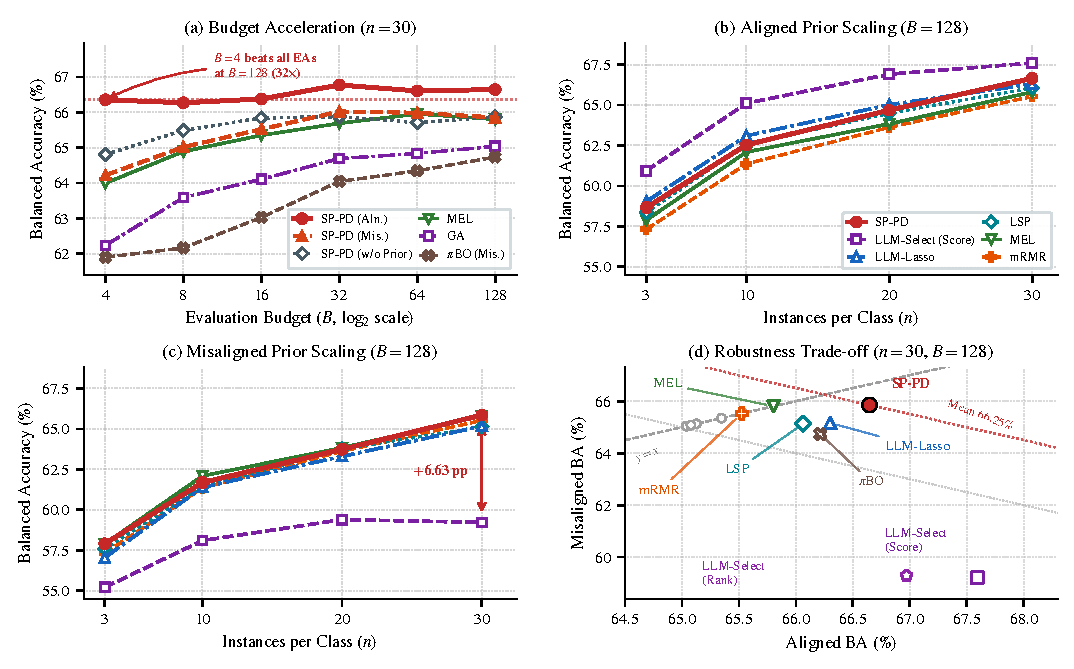
\includegraphics[width=\textwidth]{figures/fig2_clinical_scaling.pdf}
\caption{Evaluation-budget acceleration, sample-size scaling, and aligned-versus-misaligned robustness trade-off on the 12 clinical datasets ($K = 4$).}
\label{fig:clinical_scaling}
\end{figure*}

Under aligned priors in Table~\ref{tab:clinical_main} and Fig.~\ref{fig:clinical_scaling}(a) and (b), the Friedman test confirms significant differences across all training sizes, from $p = 2.4 \times 10^{-5}$ at $n = 3$ to $p = 0.011$ at $n = 30$. In Fig.~\ref{fig:clinical_scaling}(a), a single offline prior markedly accelerates early-budget search at $n = 30$. By $B = 4$, SP-PD reaches 66.36\%, ahead of SP-PD without prior by 1.55 percentage points, MEL by 2.36 percentage points, and GA by 4.13 percentage points. This $B = 4$ accuracy already exceeds every evolutionary and Bayesian baseline at $B = 128$. By $B = 128$, SP-PD reaches 66.65\%, significantly outperforming GA, EDA, mRMR, ReliefF, and L1-LR while surpassing all data-driven and hybrid baselines including $\pi$BO, LLM-Lasso, and LSP. Zero-shot prompting attains slightly higher aligned accuracy at small $n$ because ten of the 12 clinical datasets have $p \le 23$ with well-known medical feature names, avoiding finite-sample validation variance~\cite{jeong2024llmselect,zhang2025llmlasso}. LLM-Select (Score) gains an extra static edge by scoring every feature individually, requiring up to 753 native calls on voice. However, static prompts cannot adapt to higher dimensionality or cohort-specific signals: in Appendix Table~\ref{tab:app_clinical_detail}, SP-PD beats LLM-Select (Score) by 4.88 percentage points on voice and 4.22 percentage points on thyroid even under aligned priors. Meanwhile, embedded weighted-L1 baselines suffer zero-coefficient degeneration at $n = 3$, occurring in 29.2\% of folds for LLM-Lasso and 20.0\% for LSP.

When semantic priors are misaligned in Table~\ref{tab:clinical_main} and Fig.~\ref{fig:clinical_scaling}(a) and (c), zero-shot prompting cannot correct biased rankings. At $n = 30$, LLM-Select (Rank) and LLM-Select (Score) drop by 7.68 and 8.37 percentage points to rank last overall, trailing SP-PD by 24.27 percentage points on cad in Appendix Table~\ref{tab:app_clinical_detail}. Weighted-L1 hybrids avoid total collapse, yet embedding biased weights directly into the penalty leaves persistent residual error. By contrast, SP-PD combines evolutionary search with repeated-pairing prior-regularized delivery to override misleading priors rapidly. In Fig.~\ref{fig:clinical_scaling}(a), misaligned SP-PD starts at 64.22\% at $B = 4$, ahead of misaligned $\pi$BO by 2.32 percentage points, and reaches 66.02\% by $B = 32$. Across $n$, it ranks first among prior-informed methods at $n = 3$ and $n = 10$, matches LSP at $n = 20$, and reaches 65.85\% at $n = 30$, outperforming LLM-Lasso, LSP, and every prior-independent baseline including MEL. Averaged over both regimes at $n = 30$, SP-PD achieves the highest BA of 66.25\% and the best Friedman average rank of 4.25, ahead of the runner-up by two full ranks. In Fig.~\ref{fig:clinical_scaling}(d), SP-PD lies on the upper-right Pareto frontier, outperforming every adaptive and prior-independent baseline with only one offline query.

\begin{table}[!t]
\centering
\begin{threeparttable}
\caption{Cross-Classifier BA (\%) at $n = 30$}
\label{tab:clinical_downstream}
\scriptsize
\setlength{\tabcolsep}{3.6pt}
\renewcommand{\arraystretch}{1.07}
\begin{tabular}{@{}lrrr@{\hspace{8pt}}rrr@{}}
\toprule
 & \multicolumn{3}{c}{Logistic Regression} & \multicolumn{3}{c}{Random Forest} \\
\cmidrule(lr{8pt}){2-4} \cmidrule(l){5-7}
Algorithm & Aln. & Mis. & Mean & Aln. & Mis. & Mean \\
\midrule
GA                 & 64.60\rlap{\textsuperscript{*}} & -- & 64.60\rlap{\textsuperscript{*}} & 62.35\rlap{\textsuperscript{*}} & -- & 62.35\rlap{\textsuperscript{*}} \\
BPSO               & 64.95\rlap{\textsuperscript{*}} & -- & 64.95 & 62.88\rlap{\textsuperscript{*}} & -- & 62.88 \\
EDA                & 64.89 & -- & 64.89 & 62.63\rlap{\textsuperscript{*}} & -- & 62.63 \\
MEL                & 65.33 & -- & 65.33 & 63.24 & -- & 63.24 \\
mRMR               & 65.26 & -- & 65.26 & 63.44 & -- & 63.44 \\
ReliefF            & 64.91\rlap{\textsuperscript{*}} & -- & 64.91 & 62.64\rlap{\textsuperscript{*}} & -- & 62.64\rlap{\textsuperscript{*}} \\
L1-LR              & 65.17\rlap{\textsuperscript{*}} & -- & 65.17\rlap{\textsuperscript{*}} & 63.25 & -- & 63.25 \\
RF-Imp             & 65.11 & -- & 65.11 & 63.03 & -- & 63.03 \\
\midrule
$\pi$BO            & 65.71 & 64.48 & 65.09 & 63.32 & 62.40 & 62.86 \\
LLM-Lasso          & 66.11 & 64.84 & 65.48 & 64.11 & 62.74 & 63.42 \\
LSP                & 65.61 & 64.91 & 65.26 & 63.88 & 62.73 & 63.30 \\
LLM-Select (Rank)  & 66.54 & 59.02\rlap{\textsuperscript{*}} & 62.78\rlap{\textsuperscript{*}} & 63.87 & 58.65\rlap{\textsuperscript{*}} & 61.26\rlap{\textsuperscript{*}} \\
LLM-Select (Score) & \textbf{67.40} & 58.98\rlap{\textsuperscript{*}} & 63.19 & \textbf{64.50} & 58.52\rlap{\textsuperscript{*}} & 61.51 \\
\midrule
SP-PD              & 66.05 & \textbf{65.45} & \textbf{65.75} & 63.88 & \textbf{63.46} & \textbf{63.67} \\
\bottomrule
\end{tabular}
\begin{tablenotes}[flushleft]
\scriptsize
\item Aln., Mis., and Mean denote aligned, misaligned, and average BA; prior-independent baselines satisfy Aln. = Mis. = Mean.
\item[*] SP-PD significantly outperforms the baseline (Wilcoxon, $\alpha = 0.05$).
\end{tablenotes}
\end{threeparttable}
\end{table}

Cross-classifier results on independent LR and RF classifiers at $n = 30$ appear in Table~\ref{tab:clinical_downstream}. Across both classifiers, SP-PD achieves the highest misaligned BA and highest overall mean BA among all 14 algorithms, significantly outperforming GA, L1-LR on LR mean, ReliefF on RF mean, and zero-shot prompting. Under aligned priors, SP-PD surpasses all eight prior-independent baselines and $\pi$BO on both classifiers while exceeding LLM-Select (Rank) on RF. Under misaligned priors, zero-shot prompting drops by 5.2 to 8.4 percentage points, whereas SP-PD preserves full data-driven accuracy. It also outperforms LLM-Lasso and LSP on misaligned and overall means, confirming that its selected subsets generalize beyond the inner nearest-centroid evaluator.
